\documentclass[11pt]{article}
\usepackage[margin=1in]{geometry}
\usepackage{amsmath,amssymb}
\usepackage{booktabs}
\usepackage{graphicx}
\usepackage[hidelinks]{hyperref}
\usepackage{xcolor}
\usepackage{placeins}
% generated by scripts/technote_numbers.py; do not edit
\newcommand{\nRecoLL}{0.340}
\newcommand{\nRecoLLtree}{0.404}
\newcommand{\nMinosLL}{0.051}
\newcommand{\nChargeLL}{0.107}
\newcommand{\nMultLL}{0.805}
\newcommand{\nTest}{1{,}149{,}228}
\newcommand{\nWoneMax}{0.01}
\newcommand{\nWoneMuMatched}{0.004}
\newcommand{\nWoneMuUnmatched}{0.01}
\newcommand{\nWoneRecoil}{0.002}
\newcommand{\nCorrDiff}{0.008}
\newcommand{\nAUCmarg}{0.527}
\newcommand{\nAUCcond}{0.525}
\newcommand{\nAUCblockMax}{0.530}
\newcommand{\nAUCcondBlockMax}{0.522}
\newcommand{\nAUCflags}{0.497}
\newcommand{\nAUCprong}{0.519}
\newcommand{\nAUCprongCond}{0.512}
\newcommand{\nAUCvtxz}{0.543}
\newcommand{\nConfOneZero}{49\%}
\newcommand{\nConfOneOne}{43\%}
\newcommand{\nConfFourOne}{43\%}
\newcommand{\nConfMaxDiff}{0.01}
\newcommand{\nEvZero}{198{,}566}
\newcommand{\nEvSixPlus}{104}
\newcommand{\nJointAsym}{0.0007}
\newcommand{\nJointMax}{0.260}
\newcommand{\nKinFrac}{77\%}
\newcommand{\nPfitFrac}{65\%}
\newcommand{\nProngWoneMax}{0.005}
\newcommand{\nPfitLow}{24\%}
\newcommand{\nPfitPeak}{55\%}
\newcommand{\nPfitHiReal}{47\%}
\newcommand{\nPfitHiFake}{47\%}
\newcommand{\nProngsOne}{0.59}
\newcommand{\nProngsFour}{0.97}
\newcommand{\nProngsSix}{0.85}
\newcommand{\nProngsZeroReal}{0.61}
\newcommand{\nProngsZeroFake}{0.62}
\newcommand{\nEventsZeroCh}{2{,}466}
\newcommand{\nPIDevents}{61{,}558}
\newcommand{\nPIDprotonHigh}{27\%}
\newcommand{\nPIDpionHigh}{5\%}
\newcommand{\nPIDmaxDiff}{0.031}
\newcommand{\nPIDaucReal}{0.741}
\newcommand{\nPIDaucFake}{0.737}
\newcommand{\nPIDaucGap}{0.004}
\newcommand{\nScoreMedPReal}{0.27}
\newcommand{\nScoreMedPFake}{0.26}
\newcommand{\nScoreMedPiReal}{0.076}
\newcommand{\nScoreMedPiFake}{0.079}
\newcommand{\nSnapReal}{67.1\%}
\newcommand{\nSnapFake}{67.3\%}
\newcommand{\nSnapNearReal}{67.0\%}
\newcommand{\nSnapNearFake}{67.0\%}
\newcommand{\nSnapWone}{0.06}
\newcommand{\nVtxLL}{1.547}
\newcommand{\nVtxLLmarg}{1.599}
\newcommand{\nHAAUCmarg}{0.572}
\newcommand{\nHAAUCcond}{0.566}
\newcommand{\nHACalo}{0.566}
\newcommand{\nHAProng}{0.506}
\newcommand{\nHAWoneRecoil}{0.046}
\newcommand{\nHAWoneMu}{0.014}
\newcommand{\nHARecoLL}{0.268}
\newcommand{\nHAMultLL}{0.386}
\newcommand{\nHBAUCmarg}{0.575}
\newcommand{\nHBAUCcond}{0.573}
\newcommand{\nHBCalo}{0.568}
\newcommand{\nHBProng}{0.513}
\newcommand{\nHBWoneRecoil}{0.059}
\newcommand{\nHBWoneMu}{0.019}
\newcommand{\nHBRecoLL}{0.269}
\newcommand{\nHBMultLL}{0.388}
\newcommand{\nHCtlAUCmarg}{0.533}
\newcommand{\nHCtlAUCcond}{0.533}
\newcommand{\nHCtlCalo}{0.521}
\newcommand{\nHCtlProng}{0.519}
\newcommand{\nHCtlWoneRecoil}{0.005}
\newcommand{\nHCtlWoneMu}{0.007}
\newcommand{\nHCtlRecoLL}{0.342}
\newcommand{\nHCtlMultLL}{0.823}
\newcommand{\nHFullAUCmarg}{0.527}
\newcommand{\nHFullAUCcond}{0.525}
\newcommand{\nHFullCalo}{0.522}
\newcommand{\nHFullProng}{0.519}
\newcommand{\nHFullWoneRecoil}{0.002}
\newcommand{\nHFullWoneMu}{0.004}
\newcommand{\nHFullRecoLL}{0.340}
\newcommand{\nHFullMultLL}{0.805}
\newcommand{\nHtest}{32{,}449}
\newcommand{\nHtwoP}{324{,}696}
\newcommand{\nHfracTwoPtwoph}{36\%}
\newcommand{\nHfracTwoPother}{2.3\%}
\newcommand{\nHnTwoPother}{260{,}215}
\newcommand{\nHleadKETwoPTwoH}{282}
\newcommand{\nHleadKEQE}{171}
\newcommand{\nHleadKERES}{230}
\newcommand{\nHleadKEDIS}{267}


\title{A generative surrogate of MINERvA reconstruction\\ trained on the open-data Monte Carlo: performance report}
\author{L.~Wan\thanks{lwan@fnal.gov}}
\date{\today}

\begin{document}
\maketitle

\begin{abstract}
We describe and evaluate a per-event surrogate of the MINERvA reconstruction chain, trained on the open-data
Medium Energy FHC Monte Carlo. Given a generator's final-state particles and the interaction vertex, the model
samples whether a muon candidate is reconstructed, the MINOS match and charge, the reconstructed muon momentum,
vertex and calorimetric energies, and a variable-size set of hadron prongs, and writes them as a pruned
MasterAnaDev ntuple. On a held-out subrun split, gradient-boosted classifiers trained to tell surrogate from
MasterAnaDev output reach AUC \nAUCmarg{} on the event-level reconstructed quantities and
\nAUCprong{} on the prong content, with and without the truth information as additional input. All
one-dimensional marginals agree to a Wasserstein distance below 0.06 in standardised units. We document the
remaining discrepancies and the parts of the tuple that are derived rather than generated.
\end{abstract}

\tableofcontents
\listoffigures
\listoftables
\clearpage

\section{Setup}
\label{sec:setup}

\paragraph{Data.} MINERvA open data~\cite{opendata}, Medium Energy FHC standard MC, playlist 1A. The
\texttt{Truth} tree holds every generated interaction and the \texttt{MasterAnaDev} tree those with a
reconstructed muon candidate, together with a copy of the truth. The training population is CC~$\nu_\mu$
interactions with true vertex $z \ge 4000$\,mm; neutral-current, $\nu_e$ and antineutrino events are out of
scope for this version. 30 ME FHC MC files (playlist 1A), 11{,}532{,}532 CC~$\nu_\mu$ events with true vertex $z \ge 4000$~mm (41.9\% reconstructed), 87{,}999{,}212 particle tokens (10\,MeV threshold, neutrons included; 7.3 per event); subrun split 9{,}228{,}854 / 1{,}154{,}450 / 1{,}149{,}228 train / validation / test. Training: 30 epochs of the event-level model, then 16 epochs joint with the prong flow and vertex head (warm start); 3.85\,M parameters (0.57\,M encoder, 2.57\,M event flow, 0.63\,M prong flow, 0.08\,M heads); about 10 GPU-hours on one RTX~3090.


\paragraph{Inputs.} GENIE final-state particles after intranuclear FSI (\texttt{mc\_FSPart*}), dropping
neutrinos, neutrons, GENIE pseudo-particles and nuclear remnants, and hadrons with kinetic energy below
50\,MeV. Each particle enters as a species class (11 classes) and its momentum $(p_x, p_y, p_z)$; the context is
the true vertex $(x,y,z)$ and the struck nucleus $(Z, A)$. Generator-internal labels (interaction mode, $Q^2$,
$W$, $E_\nu$) are deliberately not used, so that the surrogate depends only on what physically enters the
detector and can be applied to final states from any generator.

\paragraph{Splits and metrics.} Events are split by MC subrun into train, validation and test; every number
below is on the test split. Two kinds of metric are used throughout. For one-dimensional distributions we quote
the median with the 16--84\% interval for MasterAnaDev and for one surrogate sample per event, and the
1-Wasserstein distance $W_1$ between them. For closure we train a gradient-boosted classifier
(\texttt{HistGradientBoostingClassifier}) to separate MasterAnaDev from surrogate output on half of the test
events and quote its AUC on the other half: 0.5 means indistinguishable. The classifier is run on the
reconstructed quantities alone (a marginal test) and on the reconstructed quantities together with 48 summary
features of the true final state (a conditional test); the latter is sensitive to whether the surrogate's
response is right \emph{given} the truth, not only on average.

\section{Model}
\label{sec:model}

Figure~\ref{fig:schematic} shows the architecture. One transformer set encoder over the particle tokens, with a
global token carrying the context, produces an event embedding $z$ and per-particle states $h_i$; every other
component is a head on these outputs, and the whole model is trained jointly with teacher forcing (each head
sees the true values of the quantities it is conditioned on). At sampling time the heads are hierarchical: the
hadron multiplicity $N$ is drawn first, and the prong kinematics are then generated for exactly $N$ prongs. The
prong generator is itself a second, smaller transformer over the $N$ prong tokens, so the model is not a single
transformer with output layers but an encoder followed by MLP heads, an MLP-based flow and a set-transformer
flow. The four groups of heads, in sampling order, are: (i) classification heads for the reconstruction flag, the MINOS match,
the muon charge and the prong multiplicity $N$; (ii) a vertex-plane head, because the reconstructed vertex $z$
lies exactly on one of about 200 scintillator-plane positions 22\,mm apart for \nSnapReal{} of events, which predicts
``not snapped'', ``snapped to the plane nearest the true $z$ plus $\delta\in[-3,3]$'' or ``snapped to a farther
plane'' from $z$, the flags, $N$ and the phase of the true $z$ within the plane cycle; (iii) an event flow,
conditional flow matching over 9 variables (muon momentum as a response to the true muon, vertex residual, three
calorimetric energies with exact zeros dequantised), conditioned on $z$, the flags and $N$; (iv) a prong set
flow, masked flow matching over $N$ prong tokens of 10 fields (has-kinematics flag, direction, pion- and
proton-hypothesis momenta, proton score, exiting and primary flags; binary fields dequantised), with a
permutation-equivariant velocity network that self-attends over prongs and cross-attends the particle states,
conditioned on $z$, the flags, $N$ and the event-flow sample. A decoder inverts the transforms, snaps the vertex
when the class head says so, and fills the pion, proton and secondary-proton blocks of the tuple through the
prong table. Two calorimetric branches, \texttt{recoil\_passivecorrected} and \texttt{hadron\_recoil}, are
deterministic MasterAnaDev calibrations of \texttt{recoil\_E} with point masses at fixed ratios and are
derived at decode time from a $z$-binned median ratio rather than generated (Section~\ref{sec:limits}).

\begin{figure}[h]\centering
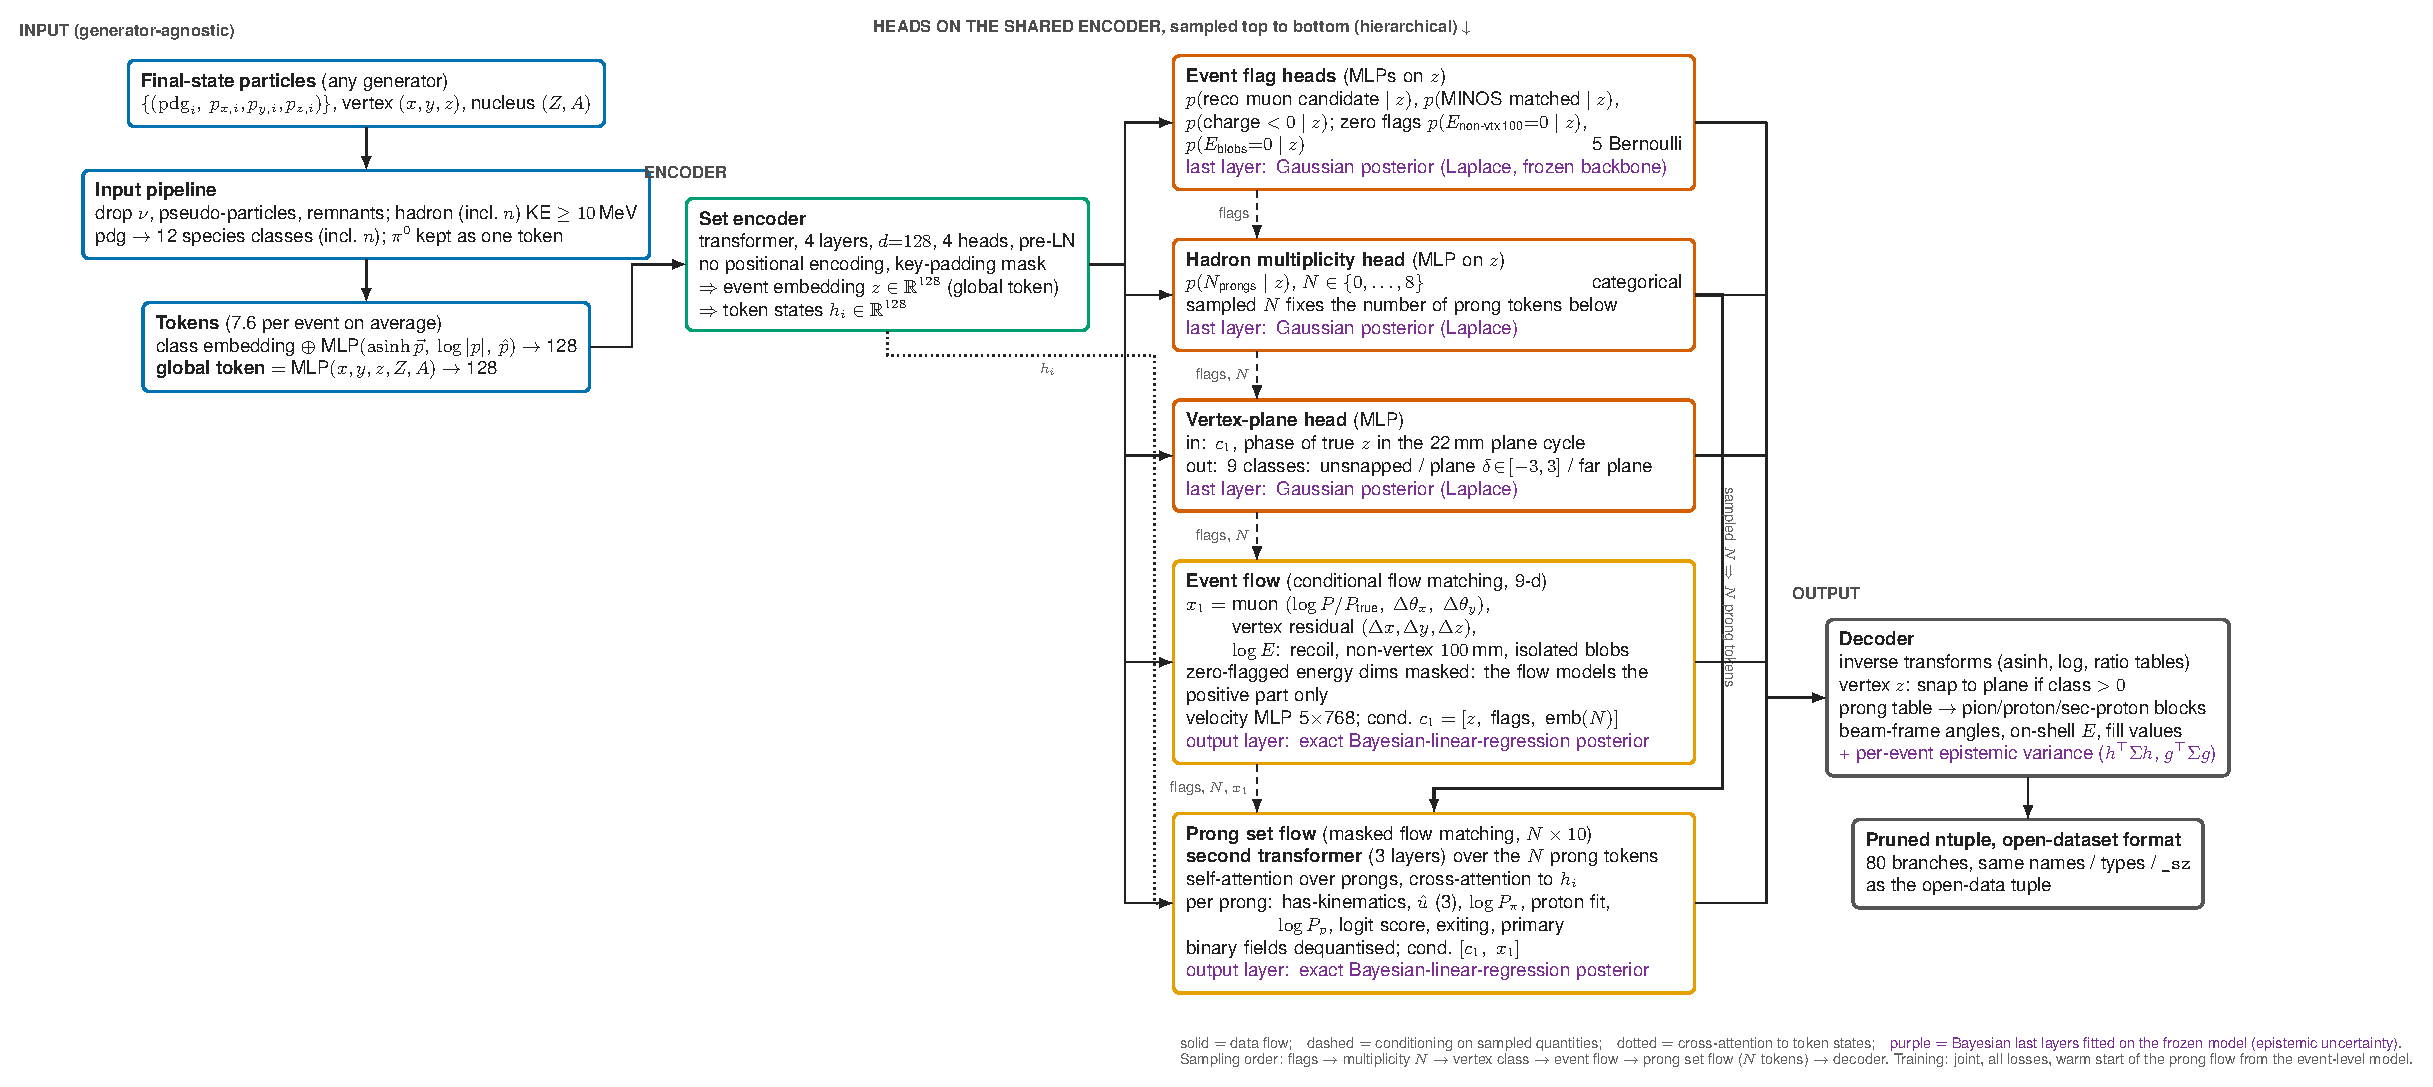
\includegraphics[width=\textwidth]{../../docs/figures/model_schematic.pdf}
\caption{Architecture of the surrogate. Solid arrows are data flow, dashed arrows conditioning on quantities
sampled by an earlier head, the dotted arrow cross-attention to the particle token states.}
\label{fig:schematic}
\end{figure}
\FloatBarrier

\section{Performance}
\label{sec:perf}

\subsection{Event classification heads}
\label{sec:heads}

Table~\ref{tab:tier0} gives the test log loss and AUC of the three binary heads against two references: the
constant-rate (marginal) predictor and a gradient-boosted tree trained on the 48 hand-built summary features
of the final state. The surrogate, which sees the raw particle set, beats the tree on every target, most
clearly for the reconstruction flag (\nRecoLL{} versus \nRecoLLtree{}). The predicted
reconstruction probability is unbiased as a function of the true hadron count (Fig.~\ref{fig:heads}, right).
Table~\ref{tab:mult} does the same for the prong multiplicity; the sampled multiplicity reproduces the
MasterAnaDev distribution (Fig.~\ref{fig:heads}, left). Figure~\ref{fig:mult-conf} shows the multiplicity
response as confusion matrices. The two truth-conditioned matrices, $P(N_\mathrm{reco} \mid n_\mathrm{true})$
for MasterAnaDev and for the surrogate, agree to \nConfMaxDiff{} in every cell: an event with one true charged hadron is
reconstructed with no prong \nConfOneZero{} of the time and with one prong \nConfOneOne{}, with four true charged hadrons the most
probable outcome is still a single prong (\nConfFourOne{}), and the surrogate reproduces this saturation. The third matrix
pairs MasterAnaDev's count with one surrogate draw for the same event (Table~\ref{tab:mult-conf}); since
reconstruction is stochastic the two draws need not coincide, and the matrix should be read as a check that the
surrogate's count is correlated with the real one through the truth, which it is, not as an accuracy.

The asymmetry of Table~\ref{tab:mult-conf} deserves a word, because it looks like a bias: events that
MasterAnaDev reconstructed with three or more prongs are given one or two prongs by the surrogate most of the
time, while the reverse rows are nearly diagonal. It is regression to the mean in the statistical sense. Given
the truth $X$, the real count and the surrogate draw are two independent realisations of the same conditional
distribution $p(N \mid X)$ if the surrogate is right; an event that happened to come out with four prongs is,
in most cases, an event for which $p(4 \mid X)$ is small, so a second draw most probably returns to one or
two. Row normalisation then divides very unequal row totals (\nEvZero{} events at $N=0$ against \nEvSixPlus{} at $N \ge 6$)
and produces the asymmetric appearance. Two checks confirm this reading (Fig.~\ref{fig:conf-sym}). First, if the
two draws are exchangeable the \emph{joint} matrix must be symmetric, and it is: the largest asymmetry
$|J_{ij} - J_{ji}|$ is \nJointAsym{} against a largest entry of \nJointMax{}. Second, two independent surrogate draws
for the same events give a row-normalised matrix with the same asymmetry as MasterAnaDev-versus-surrogate,
to within 0.01 in every populated cell; MasterAnaDev re-run with a different random seed would produce the same
picture against itself. The generative model is therefore expected to agree distribution by distribution and
conditional by conditional, which it does (Fig.~\ref{fig:mult-conf}, left and centre), and not event by event.

\begin{figure}[h]\centering
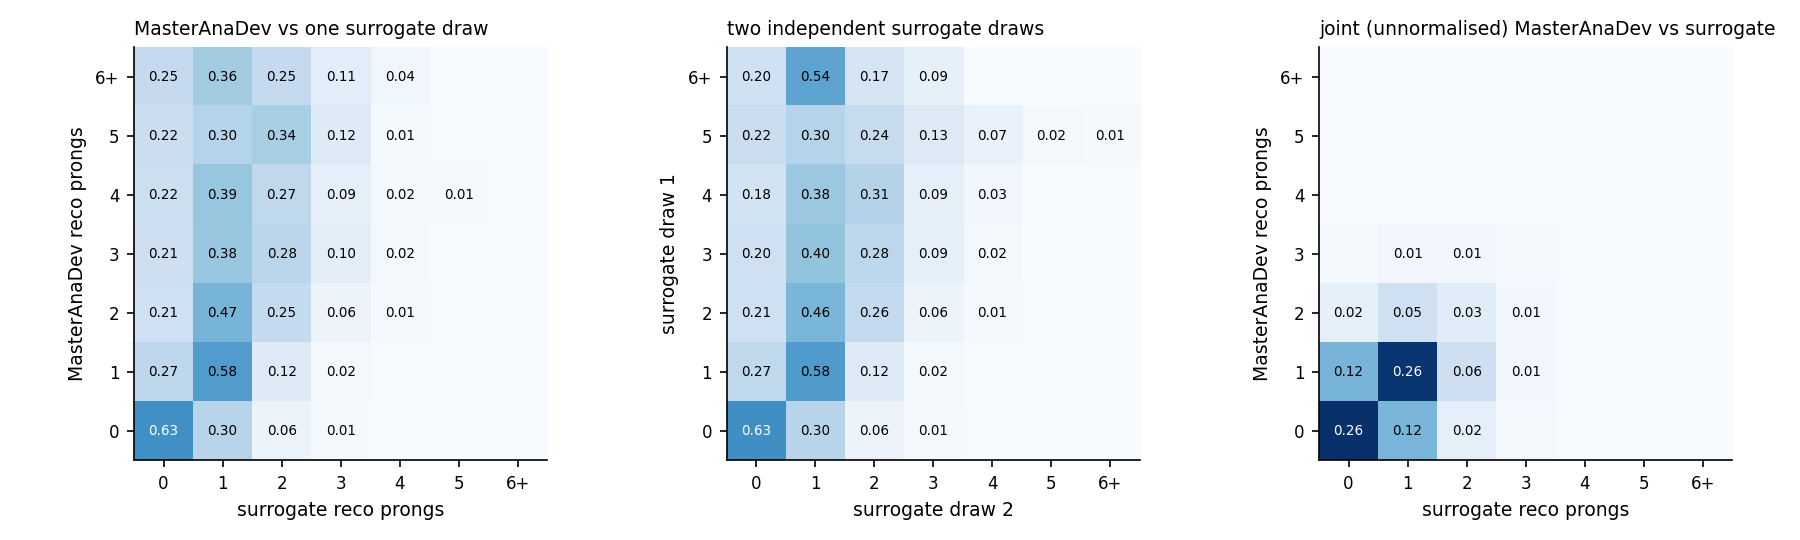
\includegraphics[width=\textwidth]{../m3_1A/figures/m3_confusion_symmetry.png}
\caption{Why the event-by-event matrix is asymmetric. Left: MasterAnaDev versus one surrogate draw,
row-normalised. Centre: two independent surrogate draws for the same events, row-normalised, showing the same
asymmetry. Right: the joint (unnormalised) MasterAnaDev-versus-surrogate matrix, symmetric to \nJointAsym{}.}
\label{fig:conf-sym}
\end{figure}

\begin{table}[h]\centering
\begin{tabular}{lccccc}
\toprule
Target & marginal & tree baseline & surrogate & AUC tree & AUC surrogate \\
\midrule
reconstructed & 0.6800 & 0.4036 & 0.3389 & 0.896 & 0.925 \\
MINOS matched $\mid$ reco & 0.5185 & 0.0869 & 0.0507 & 0.991 & 0.995 \\
negative charge $\mid$ matched & 0.1424 & 0.1078 & 0.1067 & 0.832 & 0.866 \\
\bottomrule
\end{tabular}

\caption{Binary heads: test log loss (lower is better) and AUC for the marginal predictor, the tree baseline on
summary features, and the surrogate.}
\label{tab:tier0}
\end{table}

\begin{table}[h]\centering
\begin{tabular}{lccc}
\toprule
 & marginal & tree baseline & surrogate \\
\midrule
log loss & 1.0921 & 0.8634 & 0.8018 \\
accuracy & 0.443 & 0.619 & 0.646 \\
\bottomrule
\end{tabular}

\caption{Prong multiplicity head ($N \in \{0,\dots,8\}$) among reconstructed events.}
\label{tab:mult}
\end{table}

\begin{figure}[h]\centering
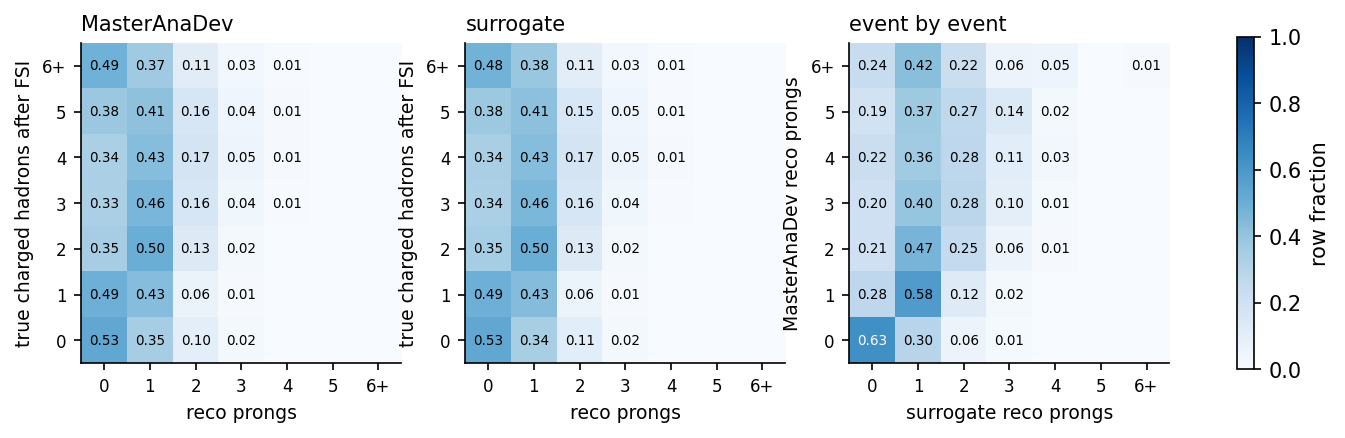
\includegraphics[width=\textwidth]{../m3_1A/figures/m3_multiplicity_confusion.png}
\caption{Prong-multiplicity confusion, row-normalised. Left and centre: reconstructed prongs versus true charged
hadrons (p, $\pi^\pm$, $K^\pm$ after FSI) for MasterAnaDev and for the surrogate. Right: MasterAnaDev's count
versus one surrogate draw for the same event.}
\label{fig:mult-conf}
\end{figure}

\begin{table}[h]\centering\small
\begin{tabular}{lccccccc}
\toprule
MasterAnaDev $N$ (events) $\backslash$ surrogate $N$ & 0 & 1 & 2 & 3 & 4 & 5 & 6+ \\
\midrule
0 (198,566) & 0.63 & 0.30 & 0.06 & 0.01 & 0.00 & 0.00 & 0.00 \\
1 (213,425) & 0.28 & 0.58 & 0.12 & 0.02 & 0.00 & 0.00 & 0.00 \\
2 (56,087) & 0.21 & 0.47 & 0.25 & 0.06 & 0.01 & 0.00 & 0.00 \\
3 (11,335) & 0.20 & 0.40 & 0.28 & 0.10 & 0.01 & 0.00 & 0.00 \\
4 (1,839) & 0.22 & 0.36 & 0.28 & 0.11 & 0.03 & 0.00 & 0.00 \\
5 (269) & 0.19 & 0.37 & 0.27 & 0.14 & 0.02 & 0.00 & 0.00 \\
6+ (104) & 0.24 & 0.42 & 0.22 & 0.06 & 0.05 & 0.00 & 0.01 \\
\bottomrule
\end{tabular}

\caption{Event-by-event confusion between MasterAnaDev's prong count (rows, with the number of test events) and
one surrogate draw (columns), row-normalised.}
\label{tab:mult-conf}
\end{table}

\begin{figure}[h]\centering
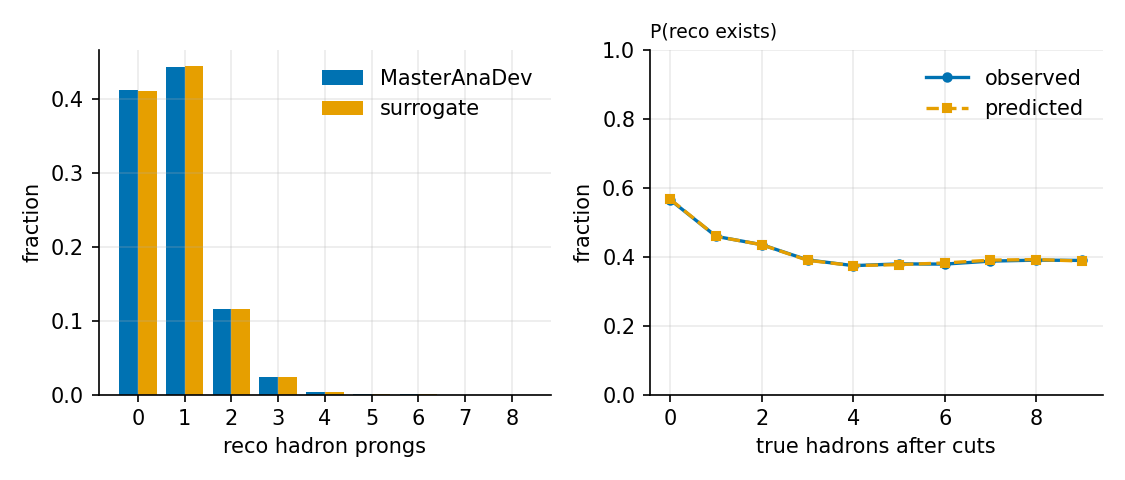
\includegraphics[width=0.75\textwidth]{../m3_1A/figures/heads_multiplicity_eff.png}
\caption{Left: reconstructed hadron-prong multiplicity, MasterAnaDev versus one surrogate sample per event.
Right: observed and predicted probability of a reconstructed muon candidate versus the number of true hadrons
after the input cuts.}
\label{fig:heads}
\end{figure}
\FloatBarrier

\subsection{Muon, vertex and calorimetry}
\label{sec:tier1}

Table~\ref{tab:tier1} lists the nine generated event-level variables in the model's standardised space.
Figure~\ref{fig:muon} shows the muon momentum response separately for MINOS-matched muons, whose ratio
$P_\mathrm{reco}/P_\mathrm{true}$ has a narrow core, and for unmatched muons, whose response is bimodal
with a spread of more than a factor of two; the surrogate reproduces both, with $W_1 = \nWoneMuMatched{}$ and
\nWoneMuUnmatched{} respectively. Figure~\ref{fig:vertex} shows the vertex residuals, whose $z$ component
carries the plane-snapping structure discussed in Section~\ref{sec:vertex}. Figure~\ref{fig:calo} shows the
calorimetric energies, including the populations at exactly zero energy reproduced by dequantisation, and the
two derived branches. Figure~\ref{fig:cond} tests the conditional behaviour: the muon response versus true
momentum and the recoil energy versus true hadronic kinetic energy follow MasterAnaDev in median and 16--84\%
band over the full range.
Figure~\ref{fig:corr} compares the correlation matrices of the nine variables; the largest difference in any
coefficient is \nCorrDiff{}.

\begin{table}[h]\centering\small
\resizebox{\textwidth}{!}{\begin{tabular}{lccc}
\toprule
Variable (model space) & MasterAnaDev median [16\%, 84\%] & surrogate median [16\%, 84\%] & $W_1$ \\
\midrule
log\_P\_ratio & -0.000 [-1.494, 1.037] & -0.003 [-1.489, 1.035] & 0.0033 \\
dtheta\_x & -0.000 [-1.165, 1.167] & 0.002 [-1.161, 1.161] & 0.0046 \\
dtheta\_y & 0.003 [-1.130, 1.190] & 0.001 [-1.132, 1.186] & 0.0065 \\
dvtx\_x & 0.001 [-1.100, 1.098] & -0.004 [-1.110, 1.093] & 0.0075 \\
dvtx\_y & -0.001 [-1.134, 1.096] & 0.001 [-1.131, 1.095] & 0.0034 \\
dvtx\_z & 0.001 [-0.897, 1.655] & 0.005 [-0.894, 1.647] & 0.0053 \\
log\_recoil\_E & -0.001 [-1.127, 0.845] & -0.003 [-1.128, 0.844] & 0.0028 \\
log\_recoil\_nonvtx100 & 0.001 [-1.811, 0.780] & 0.002 [-1.808, 0.780] & 0.0024 \\
log\_nonvtx\_iso\_blobs\_E & 0.002 [-1.848, 0.632] & 0.004 [-1.848, 0.632] & 0.0041 \\
log\_P\_ratio\_minos\_ok & 0.071 [-0.763, 0.787] & 0.067 [-0.761, 0.789] & 0.0033 \\
log\_P\_ratio\_no\_minos & -2.384 [-3.743, 3.091] & -2.382 [-3.742, 3.090] & 0.0057 \\
\bottomrule
\end{tabular}
}
\caption{Event-level generated variables on reconstructed test events, in the model's robustly standardised
space; one surrogate sample per event with the flags, multiplicity and vertex class also sampled.}
\label{tab:tier1}
\end{table}

\begin{figure}[h]\centering
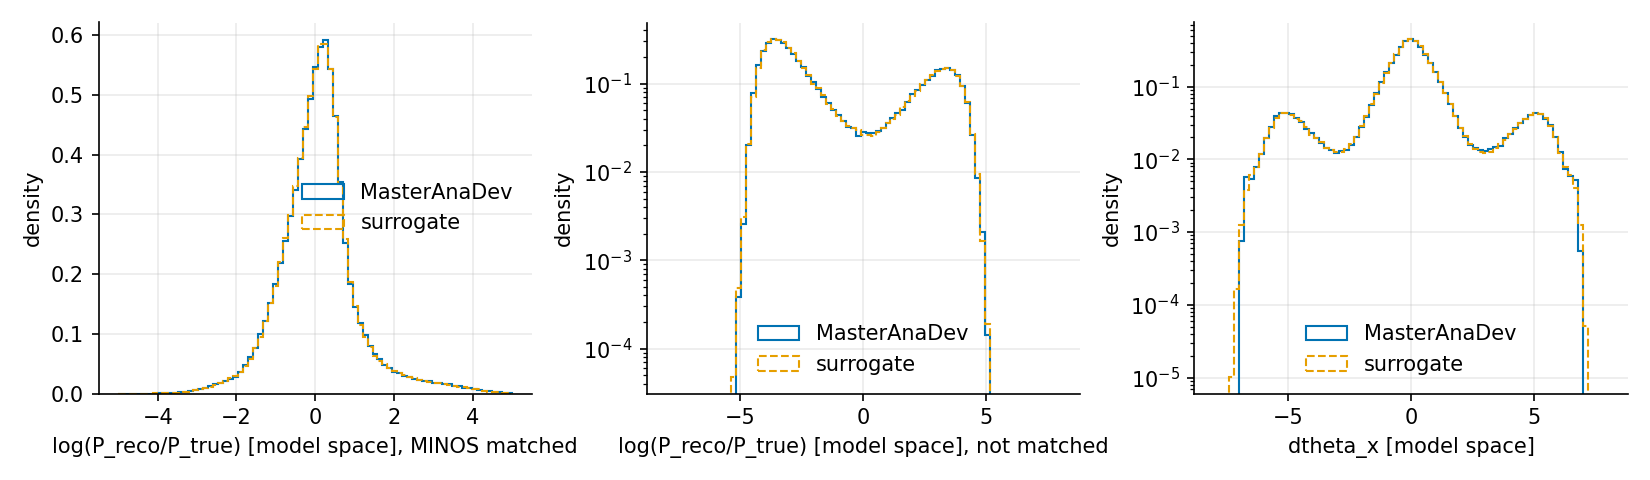
\includegraphics[width=\textwidth]{../m3_1A/figures/tier1_muon.png}
\caption{Muon response in model space: $\log(P_\mathrm{reco}/P_\mathrm{true})$ for MINOS-matched (left) and
unmatched (centre) muons, and the difference of the projected angle $\theta_x$ (right).}
\label{fig:muon}
\end{figure}

\begin{figure}[h]\centering
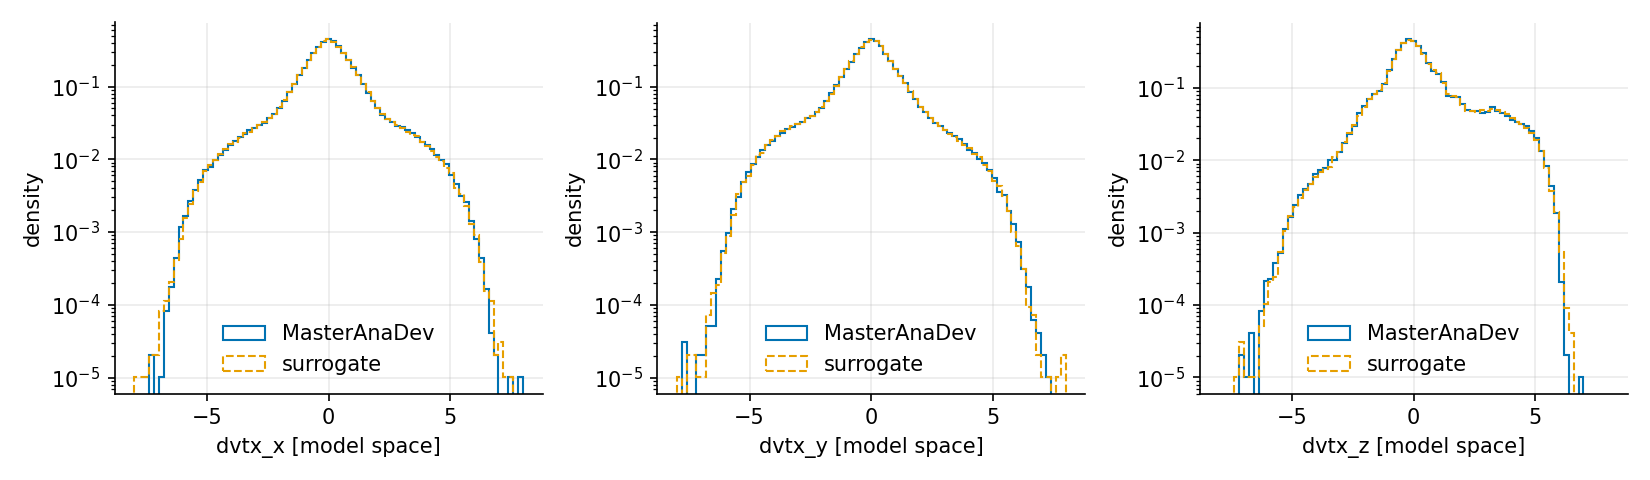
\includegraphics[width=\textwidth]{../m3_1A/figures/tier1_vertex.png}
\caption{Reconstructed-minus-true vertex residuals in model space (asinh-compressed).}
\label{fig:vertex}
\end{figure}

\begin{figure}[h]\centering
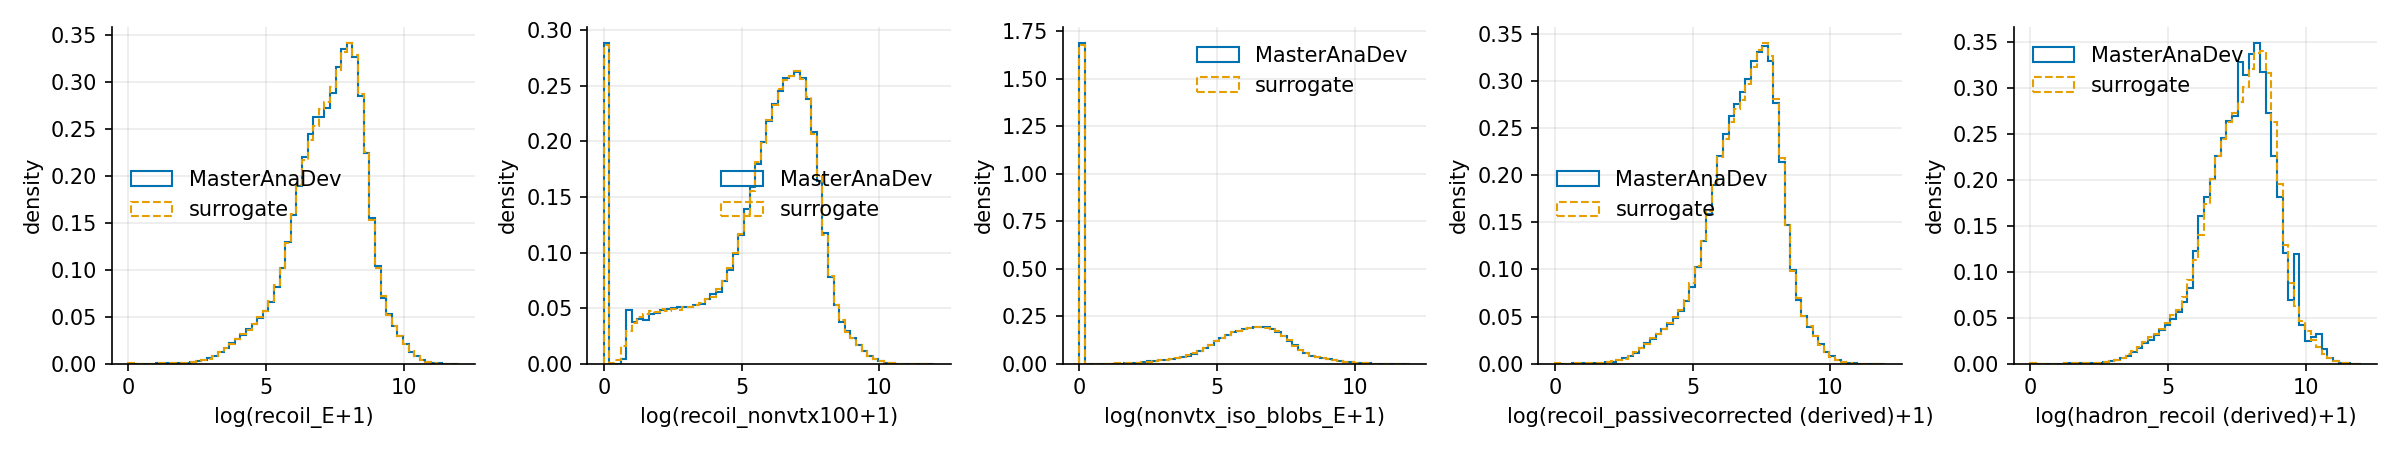
\includegraphics[width=\textwidth]{../m3_1A/figures/tier1_calorimetry.png}
\caption{Calorimetric branches, $\log(E+1)$. The first three are generated; the spike at zero is the exactly-zero
population. The last two are derived from \texttt{recoil\_E} at decode time.}
\label{fig:calo}
\end{figure}

\begin{figure}[h]\centering
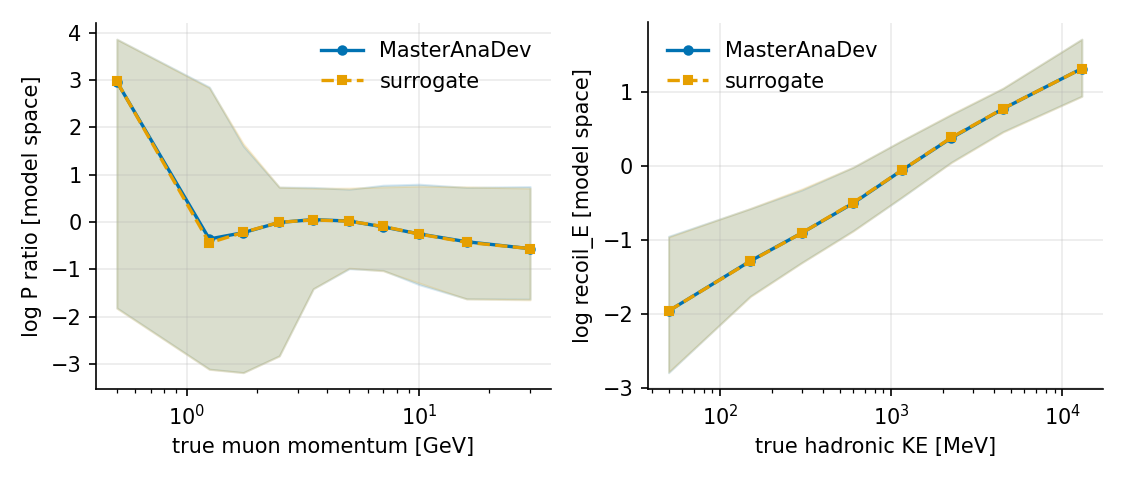
\includegraphics[width=0.75\textwidth]{../m3_1A/figures/tier1_conditionals.png}
\caption{Conditional response: median and 16--84\% band of the muon momentum ratio versus true muon momentum
(left) and of $\log E_\mathrm{recoil}$ versus true hadronic kinetic energy after cuts (right).}
\label{fig:cond}
\end{figure}

\begin{figure}[h]\centering
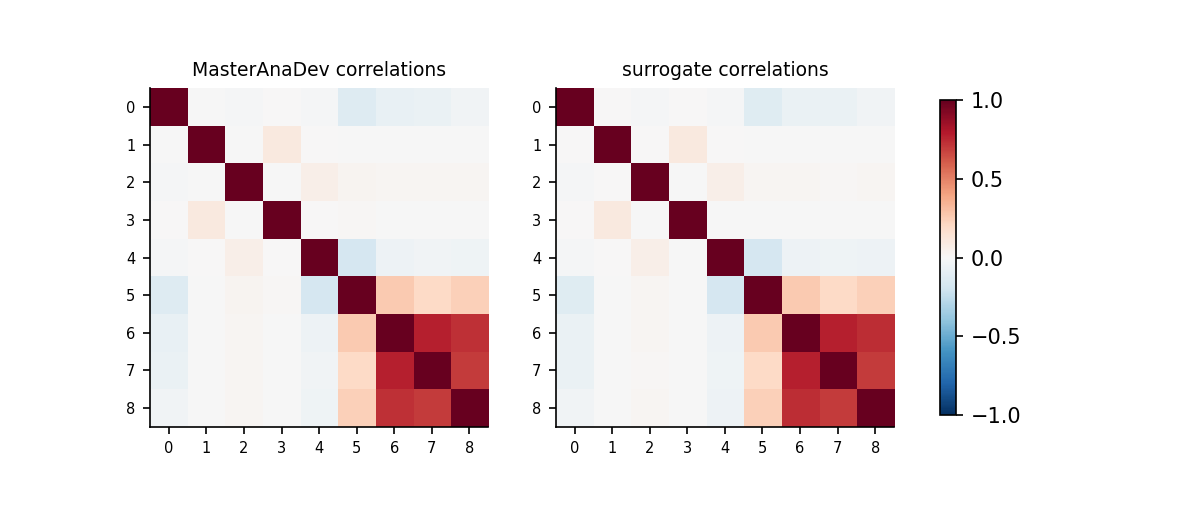
\includegraphics[width=0.75\textwidth]{../m3_1A/figures/tier1_correlations.png}
\caption{Correlation matrices of the nine event-level variables (order as in Table~\ref{tab:tier1}).}
\label{fig:corr}
\end{figure}
\FloatBarrier

\subsection{Hadron prongs}
\label{sec:prongs}

Table~\ref{tab:prongs} compares the prong-level marginals over all prongs of reconstructed test events. A
prong either carries kinematics (a direction and a pion-hypothesis momentum, \nKinFrac{} of prongs) or
nothing but its existence; \nPfitFrac{} also have a proton fit. Direction, both momentum hypotheses and the
proton score are reproduced to $W_1 \le \nProngWoneMax{}$ (Fig.~\ref{fig:prongs}), and the per-event
counts of prongs by category to within one per cent (Fig.~\ref{fig:prong-event}). No prong-to-true-particle
correspondence is generated; the flow learns the prong set given the particle set and any assignment lives
implicitly in the cross-attention.

Closure AUCs summarise agreement but hide what the hadron output looks like, so Figures~\ref{fig:prong-cond}
and~\ref{fig:prong-pid} compare physical quantities against the truth. The fraction of events with a proton fit
rises from \nPfitLow{} at a true leading-proton kinetic energy of 50--80\,MeV to \nPfitPeak{} at its peak near 300--400\,MeV and falls again
for protons above 1\,GeV, which increasingly exit or interact; the surrogate follows this curve to within one
per cent (highest bin: \nPfitHiFake{} versus \nPfitHiReal{}). The reconstructed proton-hypothesis momentum of
the leading prong tracks the truth in median and in the 16--84\% band over the same range. The mean number of
reconstructed prongs versus the true number of charged hadrons after FSI (Fig.~\ref{fig:prong-cond}, right)
shows the saturation of the reconstruction: it rises from \nProngsOne{} at one charged hadron to \nProngsFour{} at four and turns
over to \nProngsSix{} at six, and the surrogate reproduces the whole shape, including the separate curve for prongs
that carry kinematics, to within 0.01 prongs above one hadron; at zero true charged hadrons (\nEventsZeroCh{} events,
where every prong is a fake from a neutron, photon or overlay) the surrogate gives \nProngsZeroFake{} against \nProngsZeroReal{}.
Figure~\ref{fig:prong-pid} tests particle identification: the proton score of prongs in events whose leading
true hadron is a proton peaks at zero but has a shoulder at 0.8 that is absent for pion-led events, and the
surrogate reproduces both shapes (medians \nScoreMedPReal{} versus \nScoreMedPFake{} for proton-led, \nScoreMedPiReal{} versus
\nScoreMedPiFake{} for pion-led). The same figure shows the pion-hypothesis momentum in MeV and the prong angle to the
beam in degrees, where the backward population above 90$^\circ$ and the dip at 90$^\circ$ from the planar
tracking are both present in the surrogate.

Because the surrogate produces no prong-to-particle correspondence, particle identification is tested on a
sample where the correspondence is unambiguous: events with exactly one true charged hadron and exactly one
reconstructed prong (\nPIDevents{} MasterAnaDev events). Table~\ref{tab:pid} and
Figure~\ref{fig:pid} give, for each true species, the probability of each reconstruction outcome: no kinematics,
kinematics without a proton fit, proton fit with score below 0.5, proton fit with score at or above 0.5. A true
proton ends with a high proton score in \nPIDprotonHigh{} of cases against \nPIDpionHigh{} for a true $\pi^+$, and the surrogate
reproduces every entry of the matrix to within \nPIDmaxDiff{}. Using the score to separate protons from charged
pions among prongs with a proton fit gives an AUC of \nPIDaucReal{} in MasterAnaDev and \nPIDaucFake{} in the
surrogate (Fig.~\ref{fig:pid}, right), a difference of \nPIDaucGap{}.

\begin{table}[h]\centering\small
\resizebox{\textwidth}{!}{\begin{tabular}{lcccc}
\toprule
true species (events) & no kinematics & no proton fit & proton fit, score $<0.5$ & proton fit, score $\geq 0.5$ \\
\midrule
p (21,188) & 0.26 / 0.26 & 0.10 / 0.11 & 0.36 / 0.37 & 0.27 / 0.27 \\
$\pi^+$ (23,194) & 0.28 / 0.28 & 0.13 / 0.13 & 0.54 / 0.54 & 0.05 / 0.05 \\
$K^\pm$ (715) & 0.36 / 0.32 & 0.07 / 0.08 & 0.48 / 0.49 & 0.09 / 0.10 \\
\midrule
proton-vs-pion score AUC & \multicolumn{4}{c}{MasterAnaDev 0.741 / surrogate 0.737} \\
\bottomrule
\end{tabular}
}
\caption{Reconstruction outcome by true hadron species on single-hadron, single-prong events: MasterAnaDev /
surrogate row fractions, and the proton-vs-pion AUC of the proton score among prongs with a proton fit.}
\label{tab:pid}
\end{table}

\begin{figure}[h]\centering
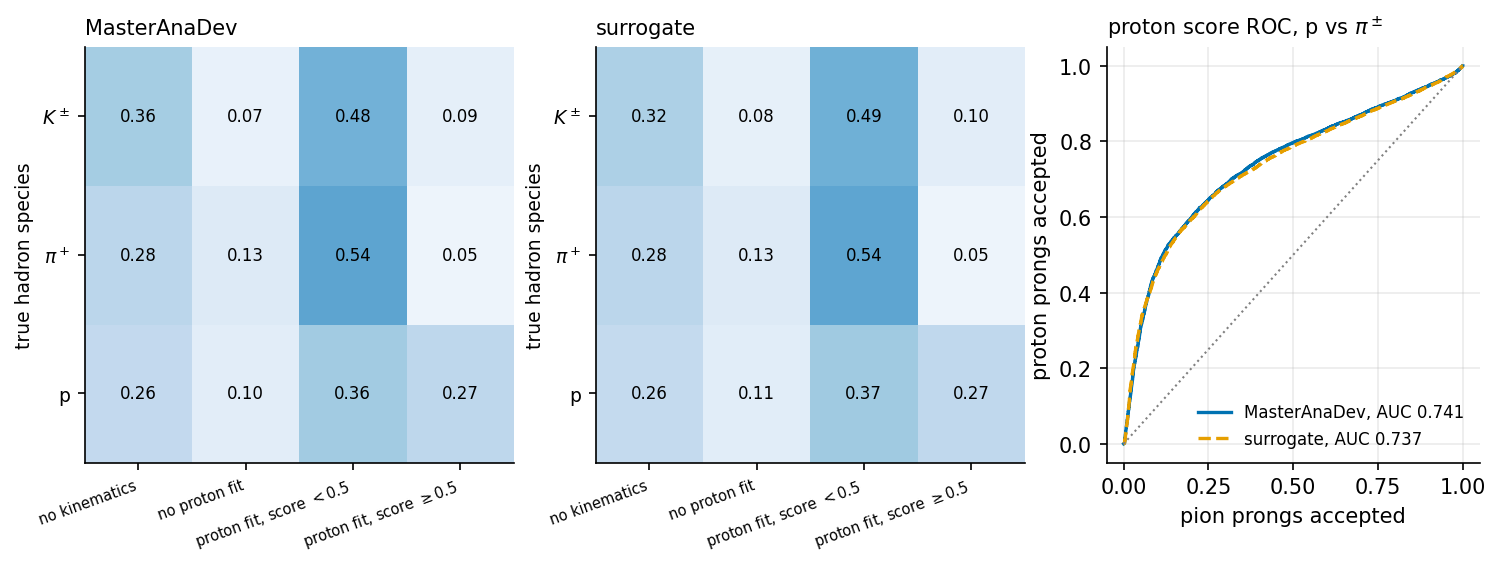
\includegraphics[width=\textwidth]{../m3_1A/figures/m3_pid_species.png}
\caption{Particle identification versus true species on single-hadron, single-prong events. Left and centre:
row-normalised outcome matrices for MasterAnaDev and the surrogate. Right: ROC curves of the proton score for
true protons against true charged pions.}
\label{fig:pid}
\end{figure}

\begin{figure}[h]\centering
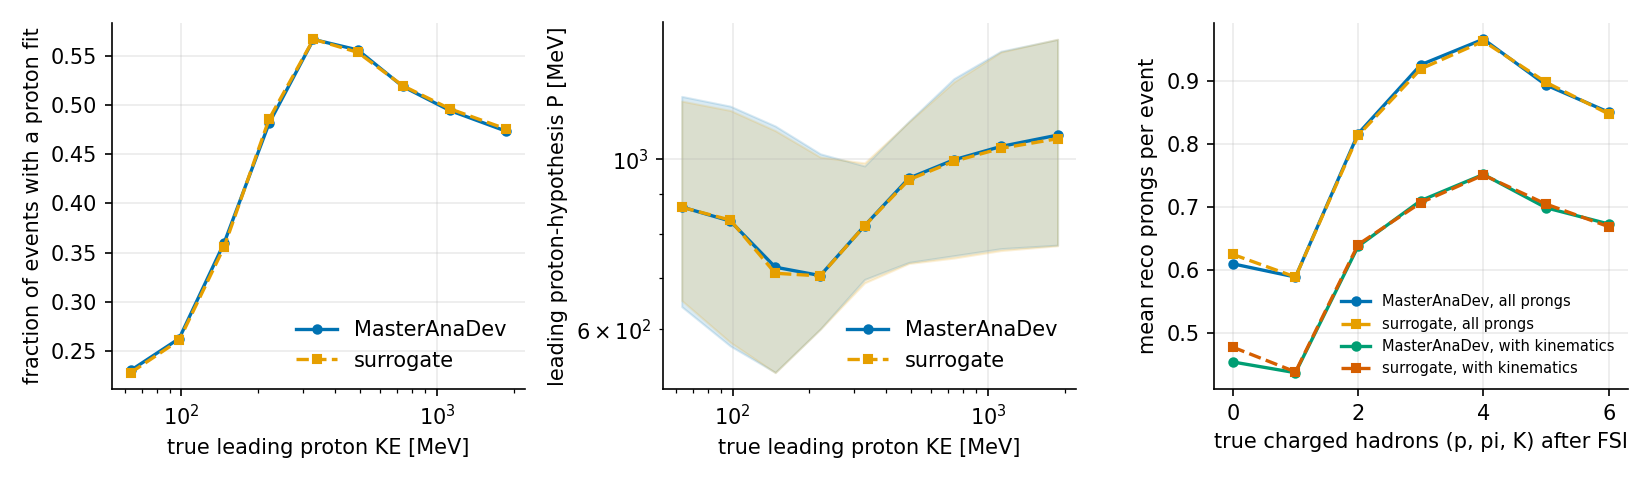
\includegraphics[width=\textwidth]{../m3_1A/figures/m3_prong_conditionals.png}
\caption{Hadron validation against the truth. Left: fraction of events with at least one proton fit versus the
true leading-proton kinetic energy. Centre: proton-hypothesis momentum of the leading prong versus the same,
median and 16--84\% band. Right: mean number of reconstructed prongs (all, and with kinematics) versus the true
number of charged hadrons after FSI.}
\label{fig:prong-cond}
\end{figure}

\begin{figure}[h]\centering
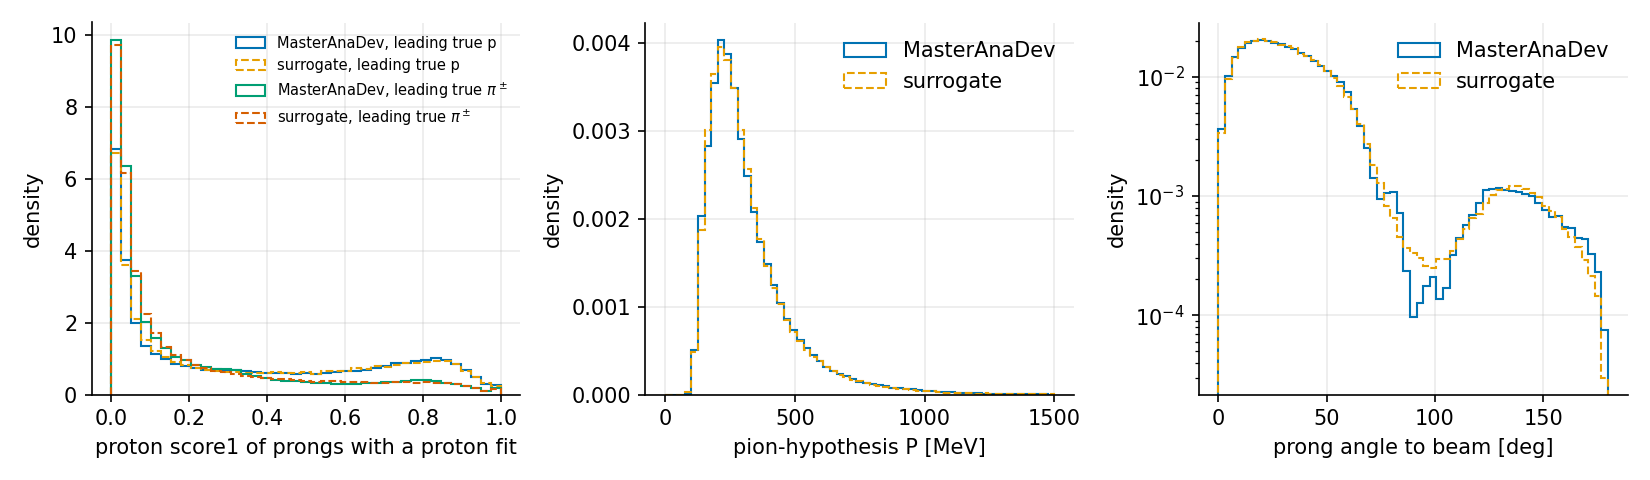
\includegraphics[width=\textwidth]{../m3_1A/figures/m3_prong_pid.png}
\caption{Left: proton score of prongs with a proton fit, for events whose leading true hadron is a proton or a
charged pion. Centre: pion-hypothesis momentum. Right: prong angle to the beam.}
\label{fig:prong-pid}
\end{figure}

\begin{table}[h]\centering
\begin{tabular}{lccc}
\toprule
Prong variable & MasterAnaDev & surrogate & $W_1$ \\
\midrule
fraction with kinematics & 0.766 & 0.766 & -- \\
fraction with proton fit & 0.652 & 0.650 & -- \\
fraction exiting & 0.214 & 0.212 & -- \\
$\theta$ [rad] & 0.535 [0.232, 0.956] & 0.530 [0.230, 0.945] & 0.0055 \\
$\log P_\pi$ & 5.615 [5.221, 6.110] & 5.615 [5.219, 6.102] & 0.0046 \\
$\log P_p$ & 6.759 [6.479, 7.077] & 6.759 [6.479, 7.072] & 0.0029 \\
proton score & 0.121 [0.019, 0.647] & 0.118 [0.019, 0.635] & 0.0032 \\
\bottomrule
\end{tabular}

\caption{Prong-level marginals: category fractions over all prongs, and median [16\%, 84\%] with $W_1$ for the
continuous fields of prongs that have the corresponding fit.}
\label{tab:prongs}
\end{table}

\begin{figure}[h]\centering
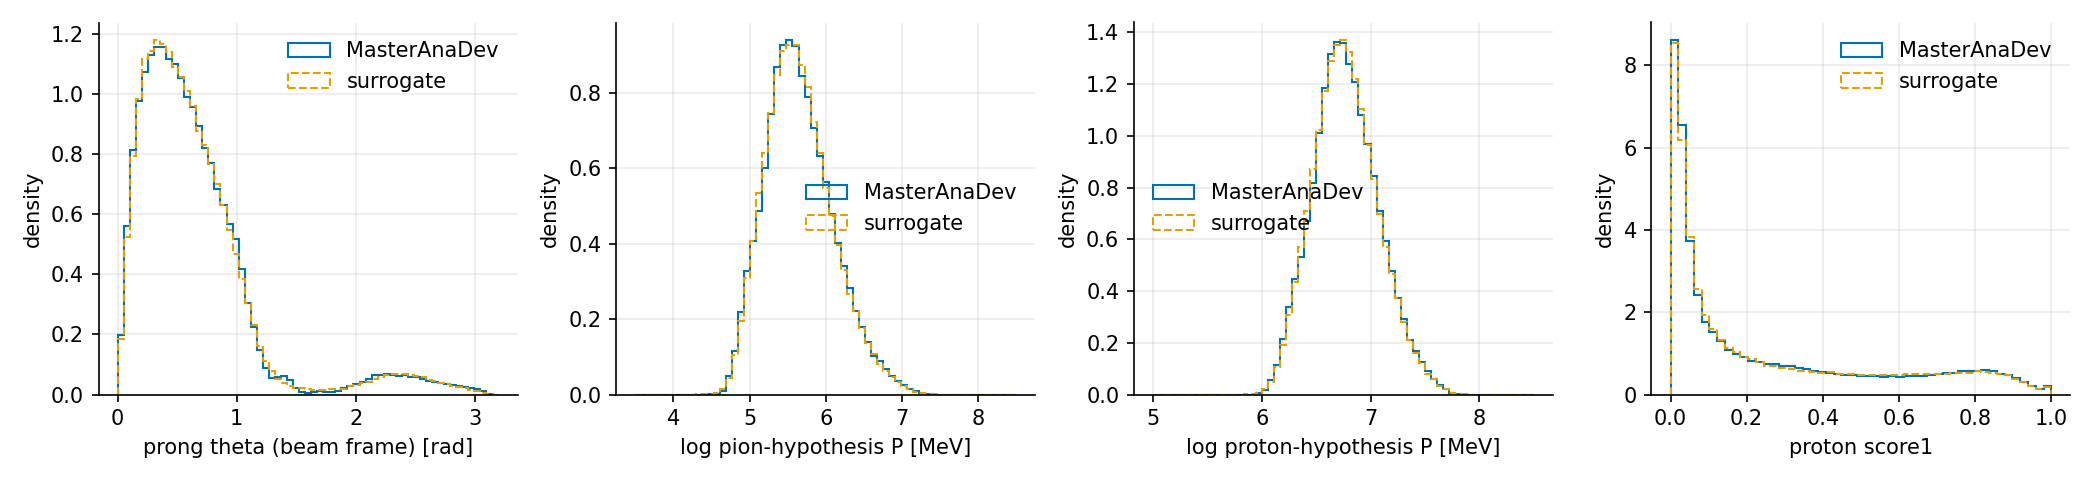
\includegraphics[width=\textwidth]{../m3_1A/figures/m3_prongs.png}
\caption{Prong direction, pion- and proton-hypothesis momenta, and proton score.}
\label{fig:prongs}
\end{figure}

\begin{figure}[h]\centering
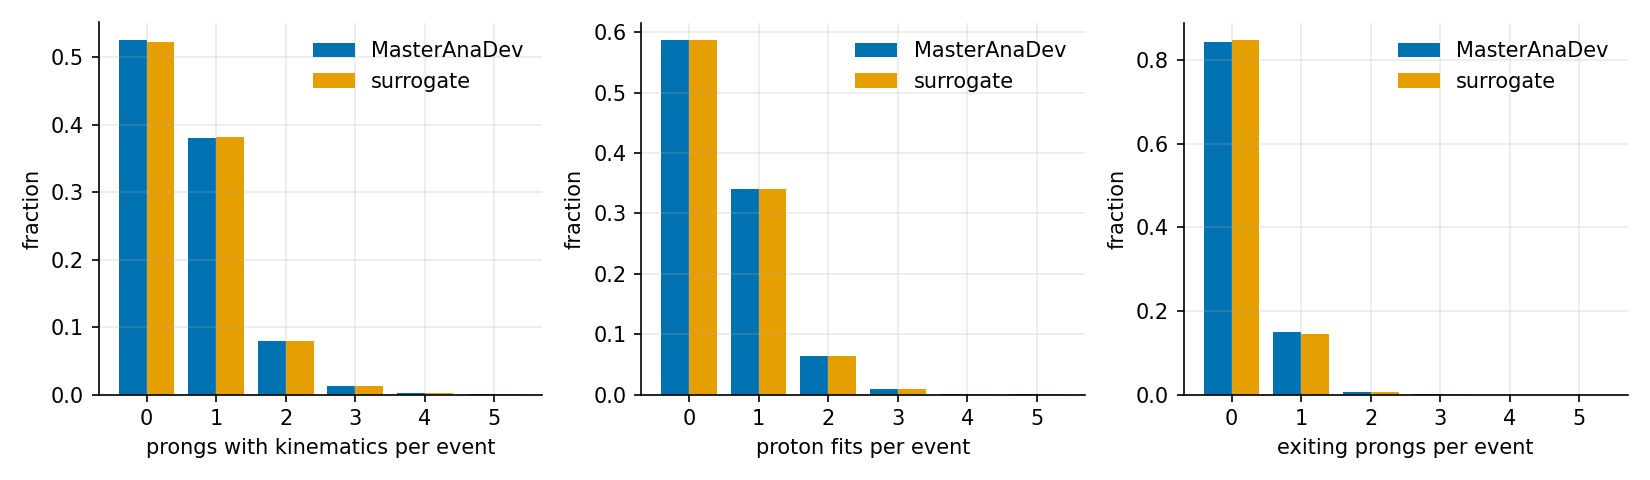
\includegraphics[width=0.9\textwidth]{../m3_1A/figures/m3_prong_event.png}
\caption{Per-event number of prongs with kinematics, with a proton fit, and exiting the detector.}
\label{fig:prong-event}
\end{figure}
\FloatBarrier

\subsection{Vertex plane}
\label{sec:vertex}

MasterAnaDev places \nSnapReal{} of reconstructed vertices within 0.1\,mm of a scintillator-plane position;
\nSnapNearReal{} of all events are within three planes of the true $z$ and the remaining snapped ones on a farther plane. The
surrogate reproduces both fractions (\nSnapFake{}, \nSnapNearFake{}) and the distribution of the
offset to the nearest plane, including the continuum of unsnapped vertices ($W_1 = \nSnapWone{}$\,mm,
Fig.~\ref{fig:vtxplane}). The class head has test log loss \nVtxLL{} against \nVtxLLmarg{} for the marginal,
evaluated with sampled flags and multiplicity as its conditions.

\begin{figure}[h]\centering
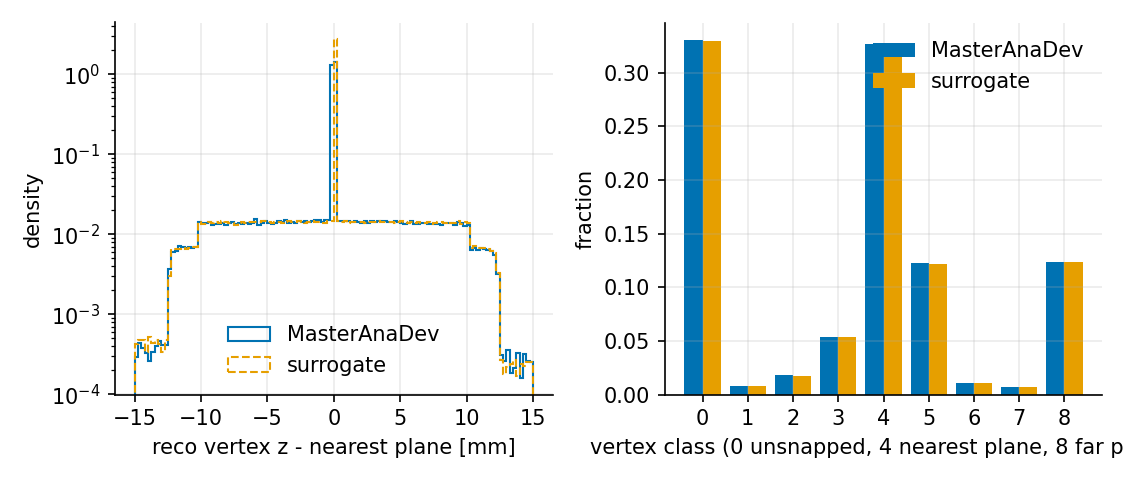
\includegraphics[width=0.75\textwidth]{../m3_1A/figures/m3_vertex.png}
\caption{Left: reconstructed vertex $z$ minus the nearest plane position; the spike at zero is the snapped
population. Right: vertex class marginals (0 unsnapped, 4 nearest plane, 8 farther plane).}
\label{fig:vtxplane}
\end{figure}
\FloatBarrier

\subsection{Closure tests}
\label{sec:closure}

Table~\ref{tab:closure} collects the classifier tests on the event-level variables and Table~\ref{tab:closure2}
those on the prongs and the vertex. On the nine event-level variables the classifier reaches AUC
\nAUCmarg{} without and \nAUCcond{} with the truth features; no block exceeds
\nAUCblockMax{} alone or \nAUCcondBlockMax{} conditionally, and the flags and multiplicity given the truth are at
\nAUCflags{}. On the prong summaries ($N$, prongs with kinematics, proton fits, exiting prongs, leading
$P_\pi$ and angle, $\sum P_\pi$, maximum score) the AUC is \nAUCprong{} and \nAUCprongCond{}; on the truth
features plus the reconstructed vertex $z$ it is \nAUCvtxz{}, the largest remaining value, from the residual
imperfection of the plane-class head. The design target for these tests was 0.55.

\begin{table}[h]\centering
\begin{tabular}{lc}
\toprule
Test & AUC \\
\midrule
real vs surrogate, reco vector only & 0.527 \\
real vs surrogate, (truth features, reco vector) & 0.525 \\
\midrule
block: muon only & 0.500 \\
block: vertex only & 0.504 \\
block: calorimetry only & 0.530 \\
truth features + flags and N only & 0.497 \\
truth features + muon & 0.498 \\
truth features + vertex & 0.498 \\
truth features + calorimetry & 0.522 \\
truth features + truth only & 0.495 \\
single variable: log\_P\_ratio & 0.501 \\
single variable: dtheta\_x & 0.501 \\
single variable: dtheta\_y & 0.502 \\
single variable: dvtx\_x & 0.501 \\
single variable: dvtx\_y & 0.499 \\
single variable: dvtx\_z & 0.503 \\
single variable: log\_recoil\_E & 0.501 \\
single variable: log\_recoil\_nonvtx100 & 0.507 \\
single variable: log\_nonvtx\_iso\_blobs\_E & 0.522 \\
\midrule
max $|\Delta$corr$|$ over the 9 generated variables & 0.008 \\
\bottomrule
\end{tabular}

\caption{Closure classifiers on the event-level variables: overall, by block, by single variable, and with the
truth features added.}
\label{tab:closure}
\end{table}

\begin{table}[h]\centering
\begin{tabular}{lc}
\toprule
Test & value \\
\midrule
vertex class log loss (marginal / head) & 1.5985 / 1.5469 \\
snapped fraction (MasterAnaDev / surrogate) & 0.670 / 0.670 \\
reco $z$ within 0.1\,mm of a plane (MasterAnaDev / surrogate) & 0.671 / 0.673 \\
\midrule
AUC: event prong summary only & 0.519 \\
AUC: truth features + prong summary & 0.512 \\
AUC: truth features + reco vertex $z$ & 0.543 \\
\bottomrule
\end{tabular}

\caption{Closure of the prong set and the vertex plane.}
\label{tab:closure2}
\end{table}
\FloatBarrier

\section{Holdout test: a 2p2h-blind surrogate}
\label{sec:holdout}

The purpose of the surrogate is to produce reconstructed-level predictions for final states the released
simulation does not contain. The first test of that claim holds out an entire interaction mode: a second model
(B) is trained from scratch with all 2p2h events (GENIE mode 8, \nHtwoP{} events, 2.8\% of the population)
removed from training and validation, while the model of Sections~\ref{sec:model}--\ref{sec:perf} (A) saw them.
Both are evaluated on the same \nHtest{} 2p2h test events against the open dataset's own reconstruction of those
events; B is also evaluated on the non-2p2h test events as a control. Neither model receives the interaction
mode as input, so the test asks whether the detector response learned from QE, resonant and deep-inelastic
final states transfers to 2p2h final states.

\paragraph{Where 2p2h sits in input space.} Figure~\ref{fig:hold-cov} shows what the blind model has to
extrapolate to. After the input cuts, 2p2h final states are pion-less: \nHfracTwoPtwoph{} have exactly two
protons, against \nHfracTwoPother{} of all other modes. The two-proton, pion-less category is nevertheless
populated in training by \nHnTwoPother{} events from other modes, mostly resonant and deep-inelastic events in
which the pion was absorbed, with softer protons (median leading-proton kinetic energy \nHleadKEQE{}\,MeV for QE
and \nHleadKERES{}\,MeV for RES against \nHleadKETwoPTwoH{}\,MeV for 2p2h). The holdout is therefore a strong
shift in composition and a moderate shift in kinematics within covered support, not a test on unseen final
states; it is the realistic case of applying the surrogate to a generator with a different 2p2h model.

\begin{figure}[h]\centering
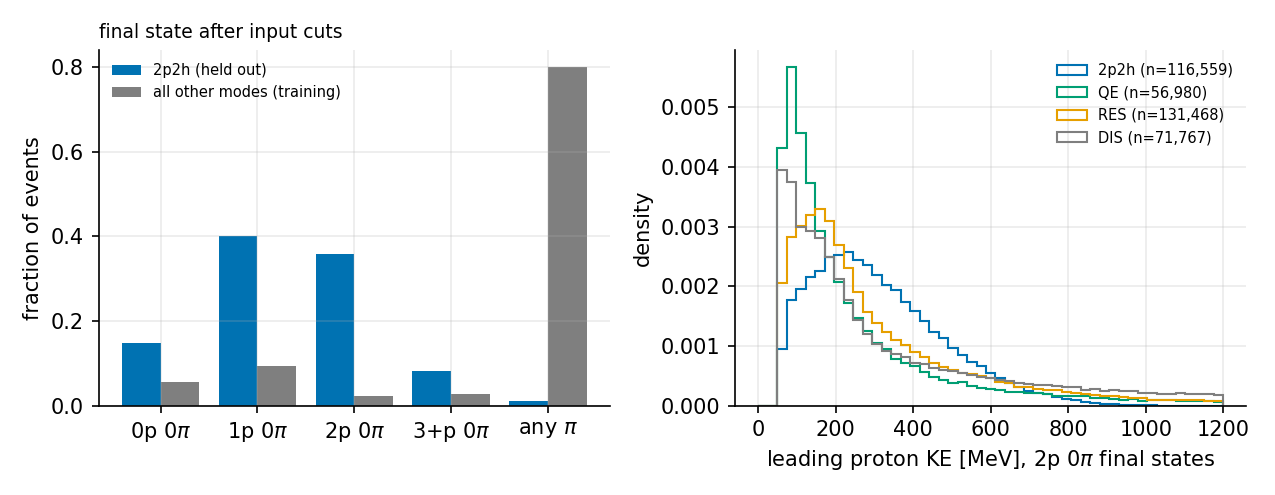
\includegraphics[width=0.9\textwidth]{../holdout_2p2h_1A/figures/holdout_input_coverage.png}
\caption{Input coverage of the held-out mode. Left: final-state category after the input cuts for 2p2h and for
all other modes. Right: leading-proton kinetic energy in two-proton, pion-less final states by interaction mode.}
\label{fig:hold-cov}
\end{figure}

\paragraph{Result.} Table~\ref{tab:holdout} compares the two models. On the 2p2h test events the blind model
is statistically indistinguishable from the model that saw them: closure AUC \nHBAUCmarg{} against
\nHAAUCmarg{} on the reconstructed quantities and \nHBAUCcond{} against \nHAAUCcond{} with the truth features,
prong closure \nHBProng{} against \nHAProng{}, identical log losses for the reconstruction flag and the
multiplicity, and $W_1$ for the recoil energy of \nHBWoneRecoil{} against \nHAWoneRecoil{}. On the control sample
B matches A's full-test performance (\nHCtlAUCmarg{} against \nHFullAUCmarg{}), so removing 2.8\% of the data
cost nothing elsewhere. Figures~\ref{fig:hold-cond}, \ref{fig:hold-eff} and~\ref{fig:hold-mult} show the three-way comparisons: the
muon response, the recoil energy versus hadronic energy and the proton momentum versus the true proton energy
(Fig.~\ref{fig:hold-cond}); the efficiency, the prong count versus true multiplicity and the proton-fit rate
(Fig.~\ref{fig:hold-eff}); and the multiplicity confusion matrices (Fig.~\ref{fig:hold-mult}), with A and B lying
on top of each other everywhere.

\begin{table}[h]\centering\small
\resizebox{\textwidth}{!}{\begin{tabular}{lcccc}
\toprule
 & A on 2p2h & B on 2p2h & B on control & A on full test \\
\midrule
reco\_exists log loss & 0.2683 & 0.2685 & 0.3418 & 0.3396 \\
MINOS log loss & 0.0191 & 0.0197 & 0.0523 & 0.0509 \\
multiplicity log loss & 0.3857 & 0.3876 & 0.8230 & 0.8050 \\
closure AUC, reco only & 0.572 & 0.575 & 0.533 & 0.527 \\
closure AUC, truth + reco & 0.566 & 0.573 & 0.533 & 0.525 \\
cond.\ AUC muon / vertex / calo & 0.479 / 0.486 / 0.566 & 0.479 / 0.489 / 0.568 & 0.498 / 0.497 / 0.521 & 0.498 / 0.498 / 0.522 \\
prong closure AUC, summary / + truth & 0.506 / 0.474 & 0.513 / 0.474 & 0.519 / 0.516 & 0.519 / 0.512 \\
$W_1$ $\log P$ ratio / $\log E_\mathrm{recoil}$ / $\log P_p$ & 0.014 / 0.046 / 0.006 & 0.019 / 0.059 / 0.014 & 0.007 / 0.005 / 0.005 & 0.004 / 0.002 / 0.004 \\
PID AUC (open dataset / surrogate) & 0.727 / 0.944 & 0.727 / 0.963 & 0.738 / 0.729 & 0.741 / 0.737 \\
test events & 32,449 & 32,449 & 1,116,740 & 1,149,228 \\
\bottomrule
\end{tabular}
}
\caption{Holdout summary. Columns: model A (trained with 2p2h) and model B (2p2h blind) on the 2p2h test
events; B on the non-2p2h control; A on the full test split. The PID AUC on 2p2h is not meaningful (three
pion-led events) and is listed only for completeness.}
\label{tab:holdout}
\end{table}

\begin{figure}[h]\centering
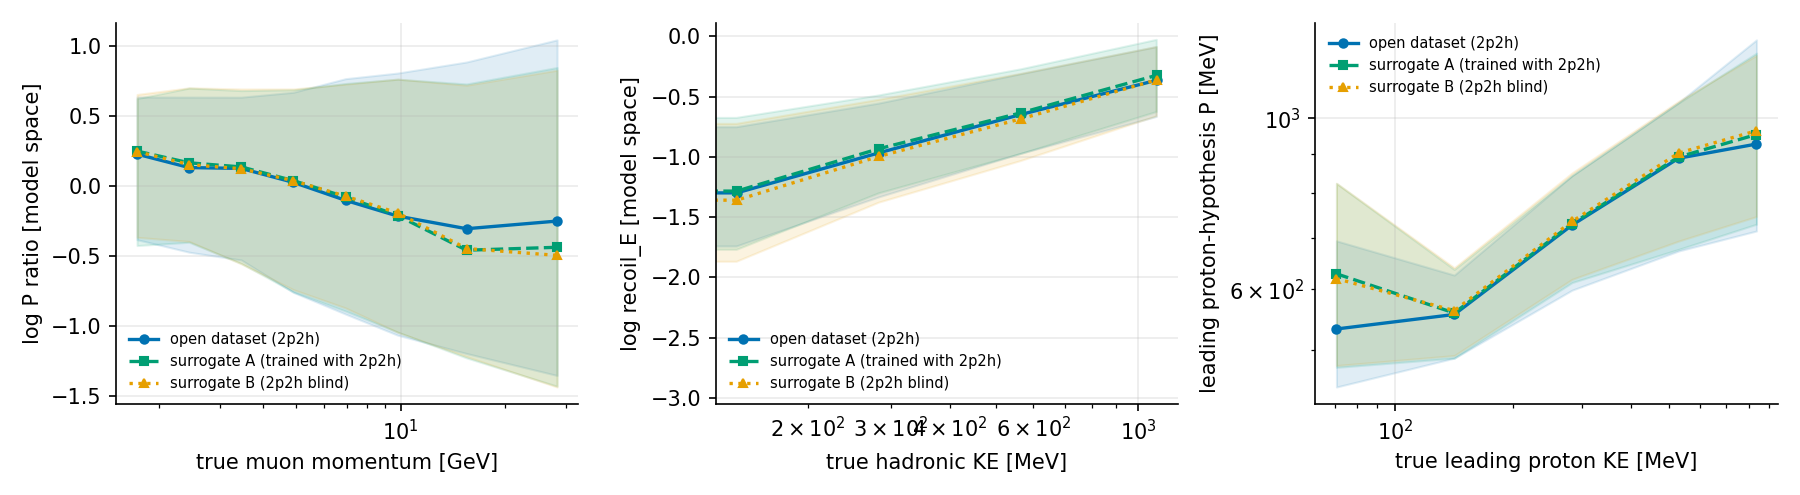
\includegraphics[width=\textwidth]{../holdout_2p2h_1A/figures/holdout_conditionals.png}
\caption{2p2h test events: muon momentum response versus true momentum, recoil energy versus true hadronic
kinetic energy, and leading proton-hypothesis momentum versus true leading-proton kinetic energy, for the open
dataset, model A and the blind model B (median and 16--84\% band).}
\label{fig:hold-cond}
\end{figure}

\begin{figure}[h]\centering
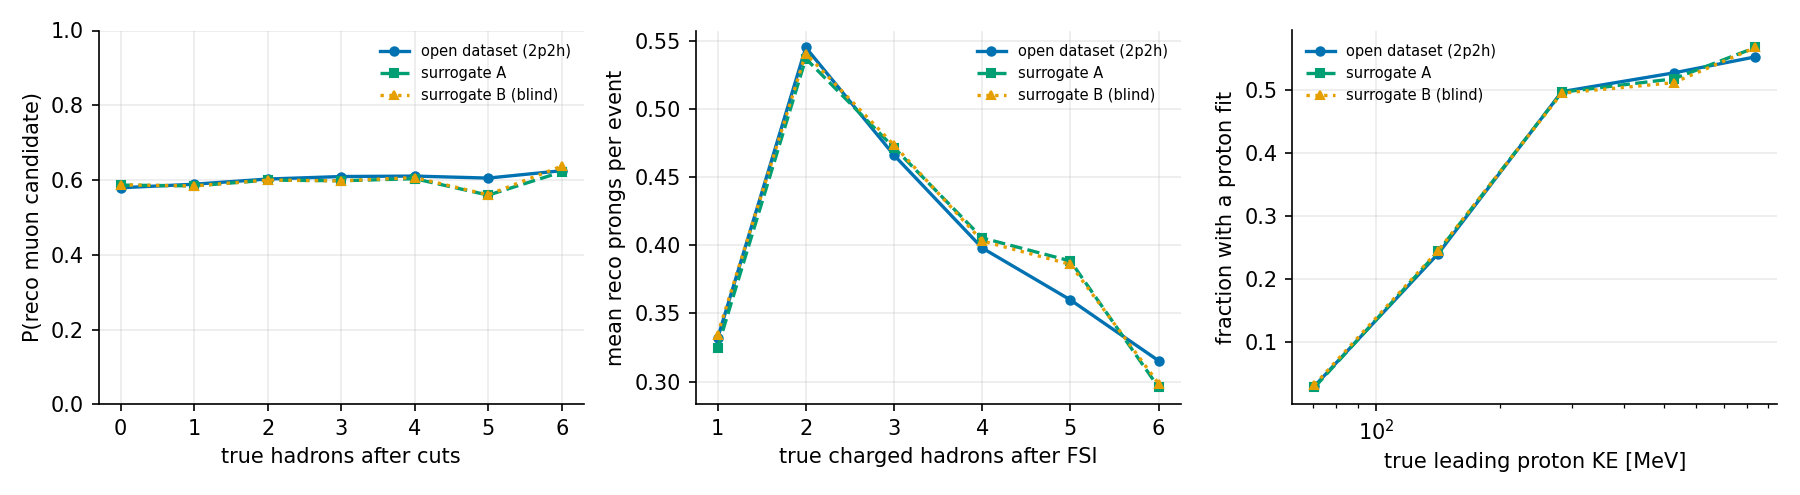
\includegraphics[width=\textwidth]{../holdout_2p2h_1A/figures/holdout_efficiency_prongs.png}
\caption{2p2h test events: reconstruction probability versus true hadron count, mean reconstructed prongs versus
true charged hadrons, and proton-fit rate versus true leading-proton kinetic energy.}
\label{fig:hold-eff}
\end{figure}

\begin{figure}[h]\centering
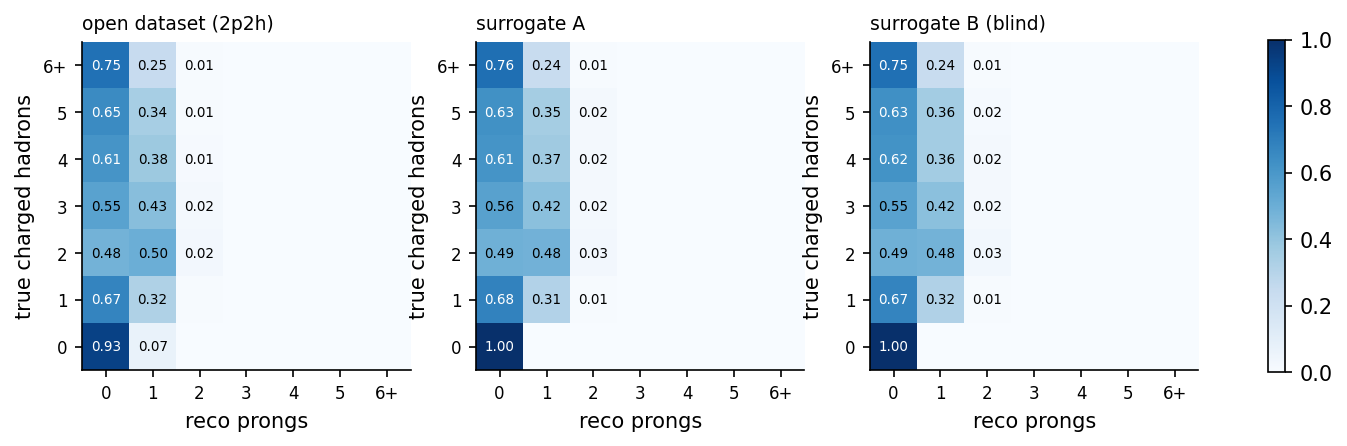
\includegraphics[width=\textwidth]{../holdout_2p2h_1A/figures/holdout_multiplicity.png}
\caption{2p2h test events: reconstructed prong multiplicity versus true charged hadrons for the open dataset,
model A and the blind model B.}
\label{fig:hold-mult}
\end{figure}

\paragraph{What the residual is.} Both models differ from the open dataset on 2p2h by about the same amount,
and more than on the full test split (AUC \nHAAUCmarg{} against \nHFullAUCmarg{}). The per-block and per-variable
classifiers locate the difference in the calorimetric block (conditional AUC \nHACalo{} for A, \nHBCalo{} for B)
and specifically in the isolated-blob energy, and the multiplicity matrices show it too: 2p2h events with no
true charged hadron after the cuts have a reconstructed prong 7\% of the time in the open dataset and never in
either surrogate. Both point at the same cause. 2p2h produces a neutron in about half of its final states, and
neutrons are dropped from the surrogate's input (design decision 2); the calorimetric activity and the
occasional fake prong they produce are then unexplained by anything the model can see, and 2p2h is the mode
where that matters most. The residual is a limitation of the input definition, not of the extrapolation, and
the obvious remedy is to let neutrons in as tokens.

\paragraph{Scope of the conclusion.} A single seed per model was trained, so differences below about 0.01 in
AUC are not resolved. The result establishes that the response transfers across a composition shift within
covered support, which is the common case for generator comparisons; it does not establish extrapolation to
final states absent from training, for which the natural next test is to hold out all two-proton, pion-less
events regardless of mode.

\section{Known limitations}
\label{sec:limits}

\begin{itemize}
\item \textbf{Derived branches.} \texttt{recoil\_passivecorrected} equals $0.6669\times$\texttt{recoil\_E} for more
  than 15\% of events and a geometry-dependent ratio otherwise; \texttt{hadron\_recoil} equals
  $1.385\times$\texttt{recoil\_E} within a MeV for a large fraction. Both are filled from \texttt{recoil\_E} and
  a median ratio in 250\,mm bins of true $z$, which drops the event-by-event scatter of the calibration (16--84\%
  widths of about 3\% and 10\%). Analyses that depend on that scatter should use \texttt{recoil\_E}.
\item \textbf{No truth-matched prongs.} The tuple's per-prong truth match is used only to validate the training
  data. A per-prong pointer head over the particle tokens would provide it.
\item \textbf{Neutrons.} Dropping neutrons from the input leaves their calorimetric activity and occasional fake
  prongs unexplained; the 2p2h holdout (Section~\ref{sec:holdout}) shows this is the dominant residual for
  neutron-rich final states. Re-admitting neutrons as tokens is the first design change to make.
\item \textbf{Scope.} CC~$\nu_\mu$, ME FHC playlist 1A, true vertex $z \ge 4000$\,mm, one training seed.
  The holdout of Section~\ref{sec:holdout} tests a composition shift within covered support; extrapolation to
  final states absent from training is not tested.
\end{itemize}

\appendix
\section{Data conventions that had to be handled}
\label{app:conv}

Every one of the following was found because a closure classifier separated real from surrogate output, not
from one-dimensional plots. They are recorded here because any surrogate of this tuple will meet them.
(1)~All angle branches are in the beam frame, rotated about $x$ by $-0.05887$\,rad; momentum components are in
the detector frame. (2)~\texttt{muon\_qp} is $-9999.9$ when there is no MINOS match, so ``negative charge'' must be
defined as matched and negative. (3)~A prong with $P=1$, $E=0$ is a direction-only sentinel. (4)~Eight of 4.8
million reconstructed events have NaN or infinite muon momenta or vertices, one a vertex coordinate of order
$10^{14}$\,mm. (5)~The two calibrated recoil branches are point masses in ratio to \texttt{recoil\_E}. (6)~The
reconstructed vertex $z$ is quantised to plane positions for \nSnapReal{} of events, and the plane chosen depends on the
true $z$'s phase within the 22\,mm cycle. (7)~Broad tails (unmatched muons, vertex residuals) must be compressed,
not clipped: clipping at $\pm 12$ robust $\sigma$ put 9--17\% of those variables on the clip boundary.

\begin{thebibliography}{9}
\bibitem{opendata} MINERvA Collaboration, Open Data Release, \url{https://minerva.fnal.gov/opendata/},
\href{https://doi.org/10.15484/3022562}{doi:10.15484/3022562}.
\end{thebibliography}

\end{document}
